% =====================================================================
%  ncwu_calc_notes_humor
%  来源：高等数学课堂笔记（幽默加料版）（YangTex 模板库 · 用户原稿全量保留版）
%  处理：仅删除编译产物 PDF / digest.lock，把 \input 递归展开为单文件；
%        正文、章节、例题、每张幻灯片、封面与参考文献一字未改。
%  字体：原稿的 macOS 字体声明全部保留，外加 \IfFontExistsTF 存在性判断；
%        在 Mac 上视觉与原 PDF 完全一致，在 Windows / Linux 上字体缺失时
%        自动跳过该声明改用默认字体，仍能正常编译。
%  编译：xelatex（目录 / 交叉引用需连续编译 2~3 遍，产品已自动处理）
% =====================================================================

% !TEX program = xelatex
% 高等数学课堂笔记 —— 格式精美、色彩多变、个性张扬（幽默加料版）
% 编译命令: xelatex advanced_math_notes.tex (需运行两遍以正确生成目录)

\documentclass[12pt,a4paper]{article}

% ==================== 宏包引入 ====================
\usepackage[UTF8,heading=false]{ctex}          % 中文支持
\usepackage{geometry}                           % 页面尺寸
\usepackage{fontawesome5}                           % 图标字体
\usepackage{colortbl}                               % 表格着色
\usepackage[most]{tcolorbox}                    % 多彩文本框
\usepackage{tikz}                               % 绘图
\usepackage{amsmath,amssymb,amsthm}             % 数学
\usepackage{mathtools}                          % 数学增强
\usepackage{fontspec}                           % 字体
\usepackage{fancyhdr}                           % 页眉页脚
\usepackage{titlesec}                           % 标题样式
\usepackage{enumitem}                           % 列表样式
\usepackage{multicol}                           % 多栏
\usepackage{pgfplots}                           % 函数绘图
\pgfplotsset{compat=1.18}
\usetikzlibrary{decorations.pathmorphing,decorations.markings,calc,shadows,shapes.geometric,arrows.meta,patterns,positioning}

% ==================== 页面设置 ====================
\geometry{
  left=18mm, right=18mm,
  top=22mm, bottom=22mm,
  headheight=15pt, footskip=25pt
}

% ==================== 色彩定义 ====================
% 个性张扬的多彩配色方案
\definecolor{MainRed}{HTML}{E63946}       % 烈焰红
\definecolor{DeepBlue}{HTML}{1D3557}      % 深海蓝
\definecolor{SkyBlue}{HTML}{457B9D}       % 天空蓝
\definecolor{MintGreen}{HTML}{2A9D8F}     % 薄荷绿
\definecolor{Sunshine}{HTML}{F4A261}      % 阳光橙
\definecolor{Royal}{HTML}{6A4C93}         % 皇家紫
\definecolor{Gold}{HTML}{E9C46A}          % 金色
\definecolor{Coral}{HTML}{E76F51}         % 珊瑚色
\definecolor{Teal}{HTML}{264653}          % 深青色
\definecolor{Pink}{HTML}{EF476F}          % 玫红
\definecolor{Lime}{HTML}{06D6A0}          % 青柠
\definecolor{Lavender}{HTML}{B5179E}      % 薰衣草紫
\definecolor{BgCream}{HTML}{FAF3E0}       % 米白底色
\definecolor{InkBlack}{HTML}{2B2D42}      % 墨黑
\definecolor{PaperWhite}{HTML}{F8F9FA}    % 纸白

% ==================== 页面背景 ====================
\pagecolor{BgCream}

% ==================== 页眉页脚 ====================
\pagestyle{fancy}
\fancyhf{}
\renewcommand{\headrulewidth}{1.5pt}
\renewcommand{\footrulewidth}{0pt}
\fancyhead[L]{\textcolor{MainRed}{\faStar~}\textcolor{DeepBlue}{\textbf{高等数学课堂笔记（幽默版）}}}
\fancyhead[R]{\textcolor{Royal}{\textbf{\thepage}}}
\fancyfoot[C]{\textcolor{SkyBlue}{\rule{0.3\textwidth}{2pt}}\\[2pt]\textcolor{Coral}{\small\textit{Keep Calm and Calculate On}}}

% ==================== 标题样式 ====================
\titleformat{\section}
  {\sffamily\Large\bfseries}
  {
\begin{tikzpicture}\fill[{MainRed}, rounded corners=4pt] (0,0) rectangle (0.9,0.9); \node[white,font=\Large\bfseries] at (0.45,0.45) {\thesection};\end{tikzpicture}}
  {1em}
  {\color{DeepBlue}}
  [\vspace{-0.1em}{\color{Sunshine}\titlerule[2pt]}\vspace{-0.2em}{\color{MintGreen}\titlerule[1pt]}]

\titleformat{\subsection}
  {\sffamily\large\bfseries\color{Royal}}
  {\thesubsection\quad}
  {0em}
  {}
  [{\color{Gold}\vspace{-5mm}\rule{8cm}{1.5pt}}]

% ==================== tcolorbox 样式定义 ====================
% 定义框 —— 深青色系
\newtcolorbox{defbox}[1]{
  enhanced, breakable,
  colback=Teal!5, colframe=Teal,
  coltitle=white, fonttitle=\bfseries\sffamily,
  title={#1},
  attach boxed title to top left={xshift=8pt,yshift=-8pt},
  boxed title style={colback=Teal, sharp corners, rounded corners=northwest},
  arc=4pt, boxrule=1.2pt,
  left=12pt, right=12pt, top=18pt, bottom=10pt,
  drop fuzzy shadow=Teal!40,
  borderline west={4pt}{0pt}{Teal}
}

% 定理框 —— 皇家紫系
\newtcolorbox{thmbox}[1]{
  enhanced, breakable,
  colback=Royal!5, colframe=Royal,
  coltitle=white, fonttitle=\bfseries\sffamily,
  title={#1},
  attach boxed title to top left={xshift=8pt,yshift=-8pt},
  boxed title style={colback=Royal, sharp corners, rounded corners=northwest},
  arc=4pt, boxrule=1.2pt,
  left=12pt, right=12pt, top=18pt, bottom=10pt,
  drop fuzzy shadow=Royal!40,
  borderline west={4pt}{0pt}{Royal}
}

% 例题框 —— 烈焰红系
\newtcolorbox{exbox}[1]{
  enhanced, breakable,
  colback=MainRed!5, colframe=MainRed,
  coltitle=white, fonttitle=\bfseries\sffamily,
  title={#1},
  attach boxed title to top left={xshift=8pt,yshift=-8pt},
  boxed title style={colback=MainRed, sharp corners, rounded corners=northwest},
  arc=4pt, boxrule=1.2pt,
  left=12pt, right=12pt, top=18pt, bottom=10pt,
  drop fuzzy shadow=MainRed!40,
  borderline west={4pt}{0pt}{MainRed}
}

% 技巧框 —— 青柠色系
\newtcolorbox{tipbox}[1]{
  enhanced, breakable,
  colback=Lime!8, colframe=Lime!70!black,
  coltitle=white, fonttitle=\bfseries\sffamily\small,
  title={#1},
  attach boxed title to top left={xshift=6pt,yshift=-7pt},
  boxed title style={colback=Lime!70!black, sharp corners, rounded corners=northwest},
  arc=3pt, boxrule=1pt,
  left=10pt, right=10pt, top=16pt, bottom=8pt,
  drop fuzzy shadow=Lime!40,
  borderline west={3pt}{0pt}{Lime!70!black}
}

% 注意框 —— 阳光橙系
\newtcolorbox{warnbox}[1]{
  enhanced, breakable,
  colback=Sunshine!10, colframe=Sunshine!80!black,
  coltitle=white, fonttitle=\bfseries\sffamily\small,
  title={#1},
  attach boxed title to top left={xshift=6pt,yshift=-7pt},
  boxed title style={colback=Sunshine!80!black, sharp corners, rounded corners=northwest},
  arc=3pt, boxrule=1pt,
  left=10pt, right=10pt, top=16pt, bottom=8pt,
  drop fuzzy shadow=Sunshine!40,
  borderline west={3pt}{0pt}{Sunshine!80!black}
}

% 公式高亮框
\newtcolorbox{formulaframe}{
  enhanced,
  colback=Gold!10, colframe=Gold!80!black,
  arc=3pt, boxrule=1pt,
  left=8pt, right=8pt, top=6pt, bottom=6pt,
  drop shadow=Gold!50
}

% 幽默段子框 —— 珊瑚色，圆润可爱
\newtcolorbox{humorbox}{
  enhanced,
  colback=Coral!8, colframe=Coral!70!black,
  arc=8pt, boxrule=1pt,
  left=8pt, right=8pt, top=6pt, bottom=6pt,
  drop fuzzy shadow=Coral!40,
  borderline west={4pt}{0pt}{Coral!80!black},
  fontupper=\itshape
}

% ==================== 自定义命令 ====================
\newcommand{\highlight}[1]{{\colorbox{Gold!40}{#1}}}
\newcommand{\redtext}[1]{{\color{MainRed}\textbf{#1}}}
\newcommand{\bluetext}[1]{{\color{DeepBlue}\textbf{#1}}}
\newcommand{\greentext}[1]{{\color{MintGreen}\textbf{#1}}}
\newcommand{\purpletext}[1]{{\color{Royal}\textbf{#1}}}
\newcommand{\orangetext}[1]{{\color{Coral}\textbf{#1}}}
\newcommand{\humor}[1]{\par\smallskip\begin{humorbox}#1\end{humorbox}\smallskip}

% 带圈数字
\newcommand{\circled}[1]{\tikz[baseline=(char.base)]\node[draw,circle,inner sep=1pt,fill=MainRed,text=white,font=\small\bfseries](char){#1};}

% ==================== 浮动体标题 ====================
\usepackage{caption}                              % 提供 \captionof 命令

% ==================== 字体形状回退 ====================
% 中文（STSong）没有“粗斜体”字形，将 bold-italic 静默回退为 bold，消除警告
\DeclareFontShape{TU}{STSong(0)}{b}{it}{<->ssub * STSong(0)/b/n}{}

% ==================== 超链接 ====================
\usepackage[hidelinks]{hyperref}

% ==================== 文档信息 ====================
\title{}
\author{}
\date{}

\begin{document}

% ==================== 封面设计 ====================
\begin{titlepage}
\begin{tikzpicture}[remember picture, overlay]
  \fill[DeepBlue] (current page.south west) rectangle (current page.north east);
  \fill[MainRed] ([yshift=-3cm]current page.north west) -- ([yshift=-3cm,xshift=6cm]current page.north west) -- ([yshift=-3.8cm,xshift=6cm]current page.north west) -- ([yshift=-3.8cm]current page.north west) -- cycle;
  \fill[Sunshine] ([yshift=-3.8cm]current page.north west) -- ([yshift=-3.8cm,xshift=9cm]current page.north west) -- ([yshift=-4.4cm,xshift=9cm]current page.north west) -- ([yshift=-4.4cm]current page.north west) -- cycle;
  \fill[MintGreen] ([yshift=-4.4cm]current page.north west) -- ([yshift=-4.4cm,xshift=12cm]current page.north west) -- ([yshift=-4.8cm,xshift=12cm]current page.north west) -- ([yshift=-4.8cm]current page.north west) -- cycle;
  \fill[Gold] ([yshift=-4.8cm]current page.north west) -- ([yshift=-4.8cm,xshift=15cm]current page.north west) -- ([yshift=-5.1cm,xshift=15cm]current page.north west) -- ([yshift=-5.1cm]current page.north west) -- cycle;
  \fill[Lime] ([yshift=-5.1cm]current page.north west) -- ([yshift=-5.1cm,xshift=18cm]current page.north west) -- ([yshift=-5.3cm,xshift=18cm]current page.north west) -- ([yshift=-5.3cm]current page.north west) -- cycle;
  \fill[Royal] ([yshift=4cm]current page.south west) -- ([yshift=4cm,xshift=7cm]current page.south west) -- ([yshift=4.6cm,xshift=7cm]current page.south west) -- ([yshift=4.6cm]current page.south west) -- cycle;
  \fill[Coral] ([yshift=4.6cm]current page.south west) -- ([yshift=4.6cm,xshift=11cm]current page.south west) -- ([yshift=5cm,xshift=11cm]current page.south west) -- ([yshift=5cm]current page.south west) -- cycle;
  \fill[Pink] ([yshift=5cm]current page.south west) -- ([yshift=5cm,xshift=15cm]current page.south west) -- ([yshift=5.2cm,xshift=15cm]current page.south west) -- ([yshift=5.2cm]current page.south west) -- cycle;
  \node[white, opacity=0.08, font=\Huge] at ([xshift=3cm,yshift=-9cm]current page.north west) {$\int_{0}^{\infty} e^{-x^2}\,dx$};
  \node[white, opacity=0.08, font=\Huge] at ([xshift=14cm,yshift=-8cm]current page.north west) {$\lim_{n\to\infty}$};
  \node[white, opacity=0.06, font=\huge] at ([xshift=5cm,yshift=-20cm]current page.north west) {$\frac{d}{dx}\left(\frac{f}{g}\right) = \frac{f'g - fg'}{g^2}$};
  \node[white, opacity=0.08, font=\Large] at ([xshift=15cm,yshift=-22cm]current page.north west) {$\sum_{n=1}^{\infty} \frac{1}{n^2} = \frac{\pi^2}{6}$};
  \node[white, opacity=0.07, font=\Huge] at ([xshift=2cm,yshift=-24cm]current page.north west) {$\nabla \times \mathbf{F}$};
  \node[white, opacity=0.06, font=\Large] at ([xshift=13cm,yshift=-11cm]current page.north west) {$\oint_C \mathbf{F}\cdot d\mathbf{r}$};
  \node[white, opacity=0.08, font=\huge] at ([xshift=4cm,yshift=-14cm]current page.north west) {$\prod_{i=1}^{n} x_i$};
  \node[white, font=\fontsize{52}{62}\selectfont\bfseries] at ([yshift=-10cm]current page.north) {高等数学};
  \node[Gold, font=\fontsize{36}{46}\selectfont\bfseries] at ([yshift=-12.5cm]current page.north) {讲~~义};
  \draw[MainRed, line width=3pt] ([yshift=-14cm,xshift=-4cm]current page.north) -- ([yshift=-14cm,xshift=4cm]current page.north);
  \draw[Lime, line width=1.5pt] ([yshift=-14.3cm,xshift=-3cm]current page.north) -- ([yshift=-14.3cm,xshift=3cm]current page.north);
  \node[white, font=\Large\itshape] at ([yshift=-16cm]current page.north) {极限 \ $\bullet$ \ 导数 \ $\bullet$ \ 微分 \ $\bullet$ \ 积分 \ $\bullet$ \ 级数};
  \node[white, font=\large] at ([yshift=-19cm]current page.north) {涵盖微积分核心知识点（附带大量吐槽）};
  \node[Gold!80, font=\normalsize] at ([yshift=-20cm]current page.north) {定义 · 定理 · 例题 · 技巧 · 注意事项 · 段子};
  \node[white, opacity=0.6, font=\small] at ([yshift=3cm]current page.south) {数学是科学之王 —— 高斯（但高数常让人想称王）};
\end{tikzpicture}
\end{titlepage}

% ==================== 开篇吐槽 ====================
\newpage
\pagenumbering{roman}
\setcounter{page}{1}
\section*{\color{DeepBlue}\centering\faBookOpen~前~言~（含免责声明）~\faBookOpen}
\begin{center}
\large\sffamily\textcolor{Royal}{欢迎来到高等数学的“游乐场”！}
\end{center}
\begin{humorbox}
本笔记在保证数学严谨性的前提下，大量注入幽默元素，旨在让您在学习时少掉几根头发。每个定理都有“人话版”，每个例题都有“生活版”。但请注意：\redtext{幽默只是调味剂，公式和证明才是主菜}。如果您只记住了段子而忘了积分，那……我也没办法。
\end{humorbox}
\vspace{1em}
\begin{center}
\begin{tikzpicture}
  \draw[step=0.5cm, color=Gold!40, very thin] (0,0) grid (4,1);
  \node[font=\small\itshape, text=DeepBlue] at (2,0.5) {数学虐我千百遍，我待数学如老友};
\end{tikzpicture}
\end{center}
\renewcommand{\contentsname}{}
\setcounter{tocdepth}{3}\thispagestyle{plain} 
{\large\sffamily\tableofcontents}

% ==================== 第一章：极限 ====================
\newpage
\pagenumbering{arabic}
\setcounter{page}{1}
\section{极限：微积分的基石}
\begin{center}\textcolor{Sunshine}{\itshape 没有极限，就没有微积分，就像没有WiFi就没有现代生活。}\end{center}

\subsection{数列的极限}

\begin{defbox}{定义 1.1 \ 数列极限的 $\varepsilon$-$N$ 定义}
设 $\{a_n\}$ 为一数列，若存在常数 $a$，使得对于任意给定的 $\varepsilon > 0$（不论多么小），总存在正整数 $N$，使得当 $n > N$ 时，一切 $a_n$ 都满足
\[
|a_n - a| < \varepsilon,
\]
则称数列 $\{a_n\}$ \textbf{收敛}于 $a$，记为
\[
\lim_{n \to \infty} a_n = a \quad \text{或} \quad a_n \to a \ (n \to \infty).
\]
若这样的常数 $a$ 不存在，则称数列 $\{a_n\}$ \textbf{发散}。
\end{defbox}
\humor{通俗版：极限就是当 $n$ 足够大时，$a_n$ 离 $a$ 要多近有多近。就像你练习投篮，出手次数够多时，落点就越来越贴近篮筐中心——数学里你能真正“投中”极限值，生活里只要坚持逼近，也一定能越来越接近自己的目标！}

% 数列收敛示意图
\begin{center}
\begin{tikzpicture}[scale=0.9]
  \draw[->, thick] (0,0) -- (10,0) node[right] {$n$};
  \draw[->, thick] (0,-0.5) -- (0,3) node[above] {$a_n$};
  \draw[dashed, MainRed, thick] (0,1.5) -- (10,1.5) node[right, text=MainRed] {$a$};
  \foreach \x in {1,...,9} {
    \pgfmathsetmacro{\y}{1.5 + 0.5*sin(\x*120)/(\x+1)}
    \fill[DeepBlue] (\x,\y) circle (2pt);
    \draw[->, Royal] (\x,\y) -- (\x+1,{1.5+0.5*sin((\x+1)*120)/(\x+2)});
  }
  \node[font=\small, text=Teal] at (5,2.8) {点列越来越靠近 $a$，但永远在抖动};
\end{tikzpicture}
\end{center}

\begin{thmbox}{定理 1.1 \ 极限的唯一性}
如果数列 $\{a_n\}$ 收敛，那么它的极限\redtext{唯一}。
\end{thmbox}
\humor{如果极限不唯一，那就像一道题同时冒出两个都对、却互相矛盾的答案——迟早要出乱子。数学可比这专一多了：收敛数列的极限，有且只有一个。}

\begin{thmbox}{定理 1.2 \ 夹逼准则（Squeeze Theorem）}
设数列 $\{x_n\}, \{y_n\}, \{z_n\}$ 满足：
\begin{enumerate}[leftmargin=2em, itemsep=2pt]
  \item $y_n \leqslant x_n \leqslant z_n$（$n = 1, 2, 3, \ldots$）；
  \item $\displaystyle\lim_{n \to \infty} y_n = \lim_{n \to \infty} z_n = a$，
\end{enumerate}
则数列 $\{x_n\}$ 的极限存在且 $\displaystyle\lim_{n \to \infty} x_n = a$。
\end{thmbox}
\humor{夹逼准则就像挤牙膏——两边一挤，中间的内容就乖乖出来了。记住：你被夹在中间时，只能听两边的。}

\begin{exbox}{例题 1.1 \ 利用夹逼准则求极限}
求 $\displaystyle\lim_{n \to \infty} \left(\frac{1}{\sqrt{n^2+1}} + \frac{1}{\sqrt{n^2+2}} + \cdots + \frac{1}{\sqrt{n^2+n}}\right)$。

\sffamily\textbf{解：}\normalfont 设 $S_n = \sum_{k=1}^{n} \frac{1}{\sqrt{n^2+k}}$，由于
\[
\frac{n}{\sqrt{n^2+n}} \leqslant S_n \leqslant \frac{n}{\sqrt{n^2+1}},
\]
而
\[
\lim_{n \to \infty} \frac{n}{\sqrt{n^2+n}} = \lim_{n \to \infty} \frac{1}{\sqrt{1+\frac{1}{n}}} = 1, \qquad
\lim_{n \to \infty} \frac{n}{\sqrt{n^2+1}} = \lim_{n \to \infty} \frac{1}{\sqrt{1+\frac{1}{n^2}}} = 1.
\]
由夹逼准则得 $\displaystyle\lim_{n \to \infty} S_n = \boxed{1}$。
\end{exbox}
\humor{这题就像你在食堂排队，左边窗口人少，右边窗口人多，你被夹在中间——最后打到的饭量一样。}

\begin{tipbox}{$\bigstar$ 实用技巧}
\textbf{夹逼准则的适用场景：}当求和或求积中各项难以单独计算时，将整体放缩到两个极限相同的表达式中。关键在于找到合适的\purpletext{上界和下界}，且二者极限相等。
\end{tipbox}

\subsection{函数的极限}

\begin{defbox}{定义 1.2 \ 函数极限的 $\varepsilon$-$\delta$ 定义}
设函数 $f(x)$ 在点 $x_0$ 的某去心邻域内有定义。若存在常数 $A$，使得对于任意 $\varepsilon > 0$，总存在 $\delta > 0$，使得当 $0 < |x - x_0| < \delta$ 时，有
\[
|f(x) - A| < \varepsilon,
\]
则称 $f(x)$ 当 $x \to x_0$ 时以 $A$ 为极限，记为 $\displaystyle\lim_{x \to x_0} f(x) = A$。
\end{defbox}
\humor{$\varepsilon$-$\delta$ 定义就像一场辩论：你说“我要多近（$\varepsilon$）”，我总能找到一个“安全范围（$\delta$）”让你满意。只要你不无理取闹，我就能陪你玩到底。}

\begin{formulaframe}
\centering
\textbf{两个重要极限：}
\[
\lim_{x \to 0} \frac{\sin x}{x} = 1 \qquad\qquad \lim_{x \to \infty}\left(1+\frac{1}{x}\right)^x = e
\]
\end{formulaframe}
\humor{这两个极限是高数界的“网红”，第一个是 $\frac{\sin x}{x}$，第二个是 $(1+\frac{1}{x})^x$，它们就像数学界的“双胞胎”，天天被拿来用，但从来不喊累。}

\begin{warnbox}{$\triangle$ 注意事项}
\begin{enumerate}[leftmargin=2em, itemsep=3pt]
  \item $\displaystyle\lim_{x \to 0}\frac{\sin x}{x} = 1$ 中的 $x$ 必须以\redtext{弧度}为单位；
  \item 第二个重要极限要求底数 $\to 1$ 且指数 $\to \infty$（$1^\infty$ 型）；
  \item 左极限 $\neq$ 右极限 $\Rightarrow$ 极限不存在。
\end{enumerate}
\end{warnbox}

\begin{exbox}{例题 1.2 \ 求 $1^\infty$ 型极限}
求 $\displaystyle\lim_{x \to 0}(1 + 3x)^{\frac{1}{x}}$。

\sffamily\textbf{解：}\normalfont 这是 $1^\infty$ 型，利用第二个重要极限：
\[
\lim_{x \to 0}(1+3x)^{\frac{1}{x}} = \lim_{x \to 0}\left[(1+3x)^{\frac{1}{3x}}\right]^{3} = e^3.
\]
故极限为 $\boxed{e^3}$。
\end{exbox}
\humor{这就像你存钱，利率是 $3x$，存 $\frac{1}{x}$ 年，最后变成 $e^3$ 倍——数学里钱生钱比现实中快多了。}

\begin{tipbox}{$\bigstar$ $1^\infty$ 型通用公式}
若 $\lim u(x) = 0$，$\lim v(x) = \infty$，则：
\[
\lim (1+u)^v = e^{\lim(u \cdot v)}
\]
即：\greentext{底数中 $1$ 后面的部分 $\times$ 指数}，取 $e$ 的幂。
\end{tipbox}

% ==================== 第二章：导数与微分 ====================
\newpage
\section{导数与微分：变化率的语言}
\begin{center}\textcolor{Sunshine}{\itshape 导数告诉你“那一刻”有多快，微分告诉你“那一小段”变了多少。}\end{center}

\subsection{导数的定义}

\begin{defbox}{定义 2.1 \ 导数}
设函数 $y = f(x)$ 在点 $x_0$ 的某邻域内有定义。若极限
\[
\lim_{\Delta x \to 0} \frac{f(x_0 + \Delta x) - f(x_0)}{\Delta x}
\]
存在，则称函数 $f(x)$ 在点 $x_0$ 处\textbf{可导}，此极限值为 $f(x)$ 在 $x_0$ 处的\textbf{导数}，记为
\[
f'(x_0), \quad \text{或} \quad y'\big|_{x=x_0}, \quad \text{或} \quad \frac{dy}{dx}\bigg|_{x=x_0}.
\]
\end{defbox}
\humor{导数就是瞬时变化率，好比你在开车时瞥一眼速度表——虽然你每时每刻速度都在变，但导数告诉你那一刻到底有多快（超速了没？）。}

% 导数与切线示意图
\begin{center}
\begin{tikzpicture}[scale=0.8]
  \draw[->, thick] (-1,0) -- (5,0) node[right] {$x$};
  \draw[->, thick] (0,-1) -- (0,4.5) node[above] {$y$};
  \draw[smooth, thick, DeepBlue, domain=-0.5:4.5, samples=100] plot (\x, {0.3*(\x-1)^2 + 1});
  \draw[MainRed, thick] (1,1) -- (3,2.2) node[right, text=MainRed] {切线 $f'(2)$};
  \node[Royal] at (2,0.5) {$\bullet$};
  \node[below] at (2,0.5) {$x_0$};
  \draw[dashed] (2,0) -- (2,1.3);
  \draw[dashed] (2,1.3) -- (0,1.3);
  \node[left] at (0,1.3) {$f(x_0)$};
  \fill (2,1.3) circle (2pt);
\end{tikzpicture}
\captionof*{figure}{导数就是切线的斜率，斜率越大，变化越猛。}
\end{center}

\begin{thmbox}{定理 2.1 \ 可导与连续的关系}
若函数 $f(x)$ 在点 $x_0$ 处可导，则 $f(x)$ 在 $x_0$ 处\redtext{连续}。\\
\textbf{反之不成立}：连续不一定可导（经典反例：$y=|x|$ 在 $x=0$ 处连续但不可导）。
\end{thmbox}
\humor{可导 $\Rightarrow$ 连续，就像有驾照 $\Rightarrow$ 会开车；但会开车不一定有驾照（比如老司机无证驾驶？）。$|x|$ 在 $0$ 处就是那个“无证驾驶”的家伙。}

\begin{formulaframe}
\centering
\textbf{基本求导公式（节选）：}
\[
\begin{array}{lll}
(C)' = 0 & (x^\mu)' = \mu x^{\mu-1} & (\sin x)' = \cos x \\[6pt]
(\cos x)' = -\sin x & (e^x)' = e^x & (\ln x)' = \dfrac{1}{x} \\[6pt]
(\tan x)' = \sec^2 x & (\arcsin x)' = \dfrac{1}{\sqrt{1-x^2}} & (\arctan x)' = \dfrac{1}{1+x^2}
\end{array}
\]
\end{formulaframe}
\humor{这些公式就像乘法口诀，必须背得滚瓜烂熟，不然考试时你会后悔的。}

\subsection{求导法则}

\begin{defbox}{定义 2.2 \ 四则运算法则}
设 $u = u(x)$，$v = v(x)$ 均可导，则：
\begin{align*}
(u \pm v)' &= u' \pm v' \\[4pt]
(Cu)' &= Cu' \quad (C\text{ 为常数}) \\[4pt]
(uv)' &= u'v + uv' \\[4pt]
\left(\frac{u}{v}\right)' &= \frac{u'v - uv'}{v^2} \quad (v \neq 0)
\end{align*}
\end{defbox}
\humor{乘法则像“你帮我、我帮你”的搭伙——$(uv)' = u'v + uv'$，各出一份力，最后加起来才完整。除法则像“分蛋糕”——分子导数乘分母，减分子乘分母导数，再除以分母的平方；别忘了分母不能为零（蛋糕可不能分给空气）。}

\begin{defbox}{定义 2.3 \ 链式法则（Chain Rule）}
设 $y = f(u)$，$u = g(x)$ 都可导，则复合函数 $y = f[g(x)]$ 的导数为：
\[
\frac{dy}{dx} = \frac{dy}{du} \cdot \frac{du}{dx} = f'(u) \cdot g'(x).
\]
\end{defbox}
\humor{链式法则就像俄罗斯套娃，一层套一层，求导时要一层层打开——从外到内，逐层剥皮。千万别漏掉任何一层，否则就像吃洋葱没剥干净。}

\begin{exbox}{例题 2.1 \ 复合函数求导}
求 $y = e^{\sin(2x)}$ 的导数。

\sffamily\textbf{解：}\normalfont 设 $y = e^u$，$u = \sin v$，$v = 2x$，由链式法则：
\[
\frac{dy}{dx} = \frac{dy}{du} \cdot \frac{du}{dv} \cdot \frac{dv}{dx} = e^u \cdot \cos v \cdot 2 = 2e^{\sin 2x}\cos 2x.
\]
\end{exbox}
\humor{这就像蛋糕塌方的连锁反应：面糊没发起来（$e$），是因为泡打粉放少了（$\sin$），放少了又是因为看错刻度（$2x$）——一环扣一环，最终“塌房”的程度就是三者的乘积。所以做数学和做蛋糕一样，每一步都得细心！}

\begin{tipbox}{$\bigstar$ 链式法则技巧}
复合函数求导的关键是\purpletext{从外到内逐层剥皮}，每层只对中间变量求导，最后将所有导数\purpletext{相乘}。不要遗漏任何一层！
\end{tipbox}

\subsection{高阶导数}

\begin{defbox}{定义 2.4 \ 高阶导数}
函数 $y = f(x)$ 的导数 $f'(x)$ 仍是 $x$ 的函数，若 $f'(x)$ 仍可导，则其导数称为 $f(x)$ 的\textbf{二阶导数}，记为 $f''(x)$ 或 $\dfrac{d^2y}{dx^2}$。一般地，$n$ 阶导数为：
\[
f^{(n)}(x) = \frac{d^n y}{dx^n} = \lim_{\Delta x \to 0} \frac{f^{(n-1)}(x+\Delta x) - f^{(n-1)}(x)}{\Delta x}.
\]
\end{defbox}
\humor{高阶导数就是导了又导，就像你剥洋葱，剥了一层又一层，直到最后眼泪汪汪（但数学不会让你哭，只会让你秃）。}

\begin{formulaframe}
\centering
\textbf{莱布尼茨公式：}
若 $u(x), v(x)$ 均 $n$ 阶可导，则
\[
(uv)^{(n)} = \sum_{k=0}^{n} \binom{n}{k} u^{(n-k)} v^{(k)}
\]
\end{formulaframe}
\humor{这个公式就像“二项式定理”的表哥，把加法换成了求导。记住它，你就可以炫耀自己懂微积分中的组合数学了。}

% ==================== 第三章：微分中值定理 ====================
\newpage
\section{微分中值定理：连接局部与整体的桥梁}
\begin{center}\textcolor{Sunshine}{\itshape 中值定理告诉你：平均速度和瞬时速度总有相遇的一刻。}\end{center}

\subsection{三大中值定理}

\begin{thmbox}{定理 3.1 \ 罗尔定理（Rolle's Theorem）}
若函数 $f(x)$ 满足：
\begin{enumerate}[leftmargin=2em, itemsep=2pt]
  \item 在闭区间 $[a, b]$ 上连续；
  \item 在开区间 $(a, b)$ 内可导；
  \item $f(a) = f(b)$，
\end{enumerate}
则至少存在一点 $\xi \in (a, b)$，使得 $f'(\xi) = 0$。
\end{thmbox}
\humor{罗尔定理说：如果你从 $a$ 点走到 $b$ 点，海拔高度一样，那么途中至少有一个时刻你是平着走的（既不上升也不下降）。这好比爬山，出发和结束在同一高度，中间肯定有个地方是平的。}

\begin{thmbox}{定理 3.2 \ 拉格朗日中值定理（Lagrange's MVT）}
若函数 $f(x)$ 满足：
\begin{enumerate}[leftmargin=2em, itemsep=2pt]
  \item 在闭区间 $[a, b]$ 上连续；
  \item 在开区间 $(a, b)$ 内可导，
\end{enumerate}
则至少存在一点 $\xi \in (a, b)$，使得
\[
f'(\xi) = \frac{f(b) - f(a)}{b - a}.
\]
\end{thmbox}
\humor{拉格朗日说：你开车从 $a$ 到 $b$，平均速度是 $\frac{f(b)-f(a)}{b-a}$，那么途中至少有一个瞬间，你的速度表正好指到这个平均速度。测速摄像头就是靠这个原理抓超速的？}

\begin{thmbox}{定理 3.3 \ 柯西中值定理（Cauchy's MVT）}
若函数 $f(x)$ 和 $g(x)$ 满足：
\begin{enumerate}[leftmargin=2em, itemsep=2pt]
  \item 在闭区间 $[a, b]$ 上连续；
  \item 在开区间 $(a, b)$ 内可导；
  \item $g'(x) \neq 0$（$x \in (a,b)$），
\end{enumerate}
则至少存在一点 $\xi \in (a, b)$，使得
\[
\frac{f'(\xi)}{g'(\xi)} = \frac{f(b) - f(a)}{g(b) - g(a)}.
\]
\end{thmbox}
\humor{柯西是拉格朗日的推广，好比你有两辆车，它们的平均速度之比等于某一时刻瞬时速度之比。这简直就是“双车并驾齐驱”的数学版本。}

\begin{tipbox}{$\bigstar$ 三大定理的关系}
\begin{center}
\begin{tikzpicture}[node distance=1.5cm and 2cm]
  \node[draw, rounded corners, fill=MainRed!15, draw=MainRed, thick, minimum width=3cm, minimum height=0.9cm, font=\small\bfseries] (cauchy) {柯西中值定理};
  \node[draw, rounded corners, fill=Sunshine!20, draw=Sunshine!80!black, thick, minimum width=3cm, minimum height=0.9cm, font=\small\bfseries, below left=of cauchy] (lagrange) {拉格朗日定理};
  \node[draw, rounded corners, fill=MintGreen!15, draw=MintGreen, thick, minimum width=3cm, minimum height=0.9cm, font=\small\bfseries, below right=of cauchy] (rolle) {罗尔定理};
  \draw[-Stealth, thick, Royal] (cauchy) -- node[above, sloped, font=\scriptsize] {$g(x)=x$} (lagrange);
  \draw[-Stealth, thick, Royal] (lagrange) -- node[below, sloped, font=\scriptsize] {$f(a)=f(b)$} (rolle);
  \node[font=\small, right=0.3cm of cauchy, text=DeepBlue] {\textbf{最一般}};
  \node[font=\small, left=0.1cm of rolle, text=DeepBlue] {\textbf{最特殊}};
\end{tikzpicture}
\end{center}
\greentext{柯西 $\supset$ 拉格朗日 $\supset$ 罗} —— 后者是前者的特例，就像矩形是正方形的爹。
\end{tipbox}

\subsection{洛必达法则}

\begin{thmbox}{定理 3.4 \ 洛必达法则（L'Hôpital's Rule）}
设函数 $f(x)$ 和 $g(x)$ 满足：
\begin{enumerate}[leftmargin=2em, itemsep=2pt]
  \item $\displaystyle\lim_{x \to a} f(x) = \lim_{x \to a} g(x) = 0$（或均为 $\infty$）；
  \item 在点 $a$ 的某去心邻域内，$f'(x)$ 和 $g'(x)$ 都存在且 $g'(x) \neq 0$；
  \item $\displaystyle\lim_{x \to a} \frac{f'(x)}{g'(x)} = A$（有限或无穷），
\end{enumerate}
则
\[
\lim_{x \to a} \frac{f(x)}{g(x)} = \lim_{x \to a} \frac{f'(x)}{g'(x)} = A.
\]
\end{thmbox}
\humor{洛必达法则就像“求极限的瑞士军刀”，什么 $\frac{0}{0}$、$\frac{\infty}{\infty}$ 都能砍，但它其实是个“富二代”——法则是由伯努利发现的，洛必达花钱买断了版权。所以用的时候别太骄傲，要感恩伯努利。}

\begin{warnbox}{$\triangle$ 洛必达法则的陷阱}
\begin{enumerate}[leftmargin=2em, itemsep=3pt]
  \item 必须先验证是 $\dfrac{0}{0}$ 型或 $\dfrac{\infty}{\infty}$ 型，否则\redtext{不能使用}；
  \item 若 $\lim \frac{f'}{g'}$ 不存在（且不为 $\infty$），\redtext{不能断定}原极限不存在——需换用其他方法；
  \item $0 \cdot \infty$、$\infty - \infty$、$1^\infty$、$0^0$、$\infty^0$ 型需先\purpletext{变形}为 $\frac{0}{0}$ 或 $\frac{\infty}{\infty}$ 型。
\end{enumerate}
\end{warnbox}
\humor{洛必达虽好，可不要贪杯哦！别看到 $\frac{0}{0}$ 就兴奋，先看看是不是真的满足条件，否则会“翻车”。}

\begin{exbox}{例题 3.1 \ 洛必达法则求极限}
求 $\displaystyle\lim_{x \to 0} \frac{x - \sin x}{x^3}$。

\sffamily\textbf{解：}\normalfont 这是 $\frac{0}{0}$ 型，连续使用洛必达法则：
\[
\lim_{x \to 0} \frac{x - \sin x}{x^3} \stackrel{L'H}{=} \lim_{x \to 0} \frac{1 - \cos x}{3x^2} \stackrel{L'H}{=} \lim_{x \to 0} \frac{\sin x}{6x} \stackrel{L'H}{=} \lim_{x \to 0} \frac{\cos x}{6} = \frac{1}{6}.
\]
故极限为 $\boxed{\dfrac{1}{6}}$。
\end{exbox}
\humor{这题用洛必达连用三次，就像连续喝三杯咖啡——最后清醒地得到 $\frac{1}{6}$。}

% ==================== 第四章：不定积分 ====================
\newpage
\section{不定积分：导数的逆运算}
\begin{center}\textcolor{Sunshine}{\itshape 积分就是找“谁是凶手”，已知凶手的长相（导数），找出真凶（原函数）。}\end{center}

\subsection{原函数与不定积分}

\begin{defbox}{定义 4.1 \ 原函数}
若在区间 $I$ 上，$F'(x) = f(x)$，则称 $F(x)$ 为 $f(x)$ 在 $I$ 上的一个\textbf{原函数}。
\end{defbox}
\humor{原函数就是那个“幕后黑手”——求导就像破案，已知导数是线索，你要找出原来的函数。}

\begin{defbox}{定义 4.2 \ 不定积分}
函数 $f(x)$ 的全体原函数称为 $f(x)$ 的\textbf{不定积分}，记为
\[
\int f(x)\,dx = F(x) + C,
\]
其中 $C$ 为\redtext{任意常数}（积分常数），$\int$ 为积分号，$f(x)$ 为被积函数，$x$ 为积分变量。
\end{defbox}
\humor{不定积分就是原函数的“全家福”，$C$ 是那个永远不定的“神秘常数”——它可以是任何数，就像你永远不知道明天会加多少班。}

\begin{formulaframe}
\centering
\textbf{基本积分公式（节选）：}
\[
\begin{array}{ll}
\displaystyle\int k\,dx = kx + C & \displaystyle\int x^\mu\,dx = \frac{x^{\mu+1}}{\mu+1} + C \quad (\mu \neq -1) \\[10pt]
\displaystyle\int \frac{1}{x}\,dx = \ln|x| + C & \displaystyle\int e^x\,dx = e^x + C \\[10pt]
\displaystyle\int \sin x\,dx = -\cos x + C & \displaystyle\int \cos x\,dx = \sin x + C \\[10pt]
\displaystyle\int \frac{1}{1+x^2}\,dx = \arctan x + C & \displaystyle\int \frac{1}{\sqrt{1-x^2}}\,dx = \arcsin x + C
\end{array}
\]
\end{formulaframe}
\humor{这些积分公式就像是求导公式的“镜像世界”，从右往左念，就是积分。}

\subsection{积分方法}

\begin{defbox}{定义 4.3 \ 换元积分法（第一类）}
设 $f(u)$ 具有原函数 $F(u)$，$u = \varphi(x)$ 可导，则：
\[
\int f[\varphi(x)]\varphi'(x)\,dx = \int f(u)\,du = F(u) + C = F[\varphi(x)] + C.
\]
\end{defbox}
\humor{换元法就像“变身术”——把复杂的积分变个形，变成简单的，积完再变回来。有点像川剧变脸。}

\begin{defbox}{定义 4.4 \ 分部积分法}
设 $u = u(x)$，$v = v(x)$ 具有连续导数，则：
\[
\int u\,dv = uv - \int v\,du
\]
\end{defbox}
\humor{分部积分就像打架，你要选谁当“$u$”（挨打的）谁当“$dv$”（打人的）。选错了，会越积越复杂，就像打架找错对手。}

\begin{tipbox}{$\bigstar$ 分部积分的 LIATE 选择法则}
选择 $u$ 的优先顺序（\purpletext{排在前面的选作 $u$}）：
\begin{itemize}[leftmargin=2em, itemsep=2pt]
  \item \textbf{L} —— 对数函数（$\ln x$）
  \item \textbf{I} —— 反三角函数（$\arcsin x, \arctan x$）
  \item \textbf{A} —— 代数函数（多项式 $x^n$）
  \item \textbf{T} —— 三角函数（$\sin x, \cos x$）
  \item \textbf{E} —— 指数函数（$e^x$）
\end{itemize}
\end{tipbox}
\humor{记住 LIATE，就像记住“红橙黄绿紫”的彩虹顺序一样——对数、反三角、代数、三角、指数，优先级依次递减。}

\begin{exbox}{例题 4.1 \ 分部积分法}
求 $\displaystyle\int x e^x\,dx$。

\sffamily\textbf{解：}\normalfont 按 LIATE 法则，选 $u = x$（代数），$dv = e^x\,dx$，则 $du = dx$，$v = e^x$：
\[
\int x e^x\,dx = xe^x - \int e^x\,dx = xe^x - e^x + C = (x-1)e^x + C.
\]
\end{exbox}
\humor{这题就像选谁当“老大”——$x$ 是代数，$e^x$ 是指数，按 LIATE，$x$ 先上，结果完美。}

\begin{exbox}{例题 4.2 \ 换元积分法}
求 $\displaystyle\int \frac{1}{\sqrt{a^2 - x^2}}\,dx$（$a > 0$）。

\sffamily\textbf{解：}\normalfont 令 $x = a\sin t$（$-\frac{\pi}{2} < t < \frac{\pi}{2}$），则 $dx = a\cos t\,dt$，
\[
\int \frac{dx}{\sqrt{a^2-x^2}} = \int \frac{a\cos t\,dt}{\sqrt{a^2 - a^2\sin^2 t}} = \int \frac{a\cos t}{a\cos t}\,dt = \int dt = t + C.
\]
回代 $t = \arcsin\frac{x}{a}$，得
\[
\int \frac{dx}{\sqrt{a^2-x^2}} = \arcsin\frac{x}{a} + C.
\]
\end{exbox}
\humor{三角换元就像用三角函数“化妆”，把根号去掉，化完妆再卸妆（回代），得到最终结果。}

% ==================== 第五章：定积分 ====================
\newpage
\section{定积分：无穷小量的累加}
\begin{center}\textcolor{Sunshine}{\itshape 定积分就是求曲线下的面积，黎曼和就是把面积切成小条，条越细越精确。}\end{center}

\subsection{定积分的概念}

\begin{defbox}{定义 5.1 \ 定积分的黎曼定义}
设函数 $f(x)$ 在 $[a, b]$ 上有界。在 $[a,b]$ 中任意插入分点 $a = x_0 < x_1 < \cdots < x_n = b$，令 $\Delta x_k = x_k - x_{k-1}$，$\lambda = \max\{\Delta x_k\}$。任取 $\xi_k \in [x_{k-1}, x_k]$，若极限
\[
\lim_{\lambda \to 0} \sum_{k=1}^{n} f(\xi_k)\,\Delta x_k
\]
存在且与分点取法及 $\xi_k$ 取法无关，则称此极限为 $f(x)$ 在 $[a,b]$ 上的\textbf{定积分}，记为
\[
\int_a^b f(x)\,dx = \lim_{\lambda \to 0} \sum_{k=1}^{n} f(\xi_k)\,\Delta x_k.
\]
\end{defbox}
\humor{黎曼和就像切披萨，切成无穷多块，每块越窄，加起来就越接近真实面积。不过你永远吃不到无穷多块，所以数学帮你想到了极限。}

% 定积分面积示意图
\begin{center}
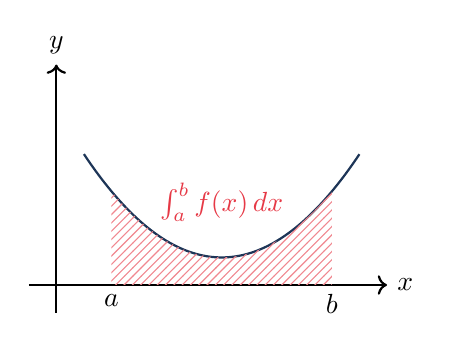
\begin{tikzpicture}[scale=0.7]
  \draw[->, thick] (-0.5,0) -- (6,0) node[right] {$x$};
  \draw[->, thick] (0,-0.5) -- (0,4) node[above] {$y$};
  \draw[smooth, thick, DeepBlue, domain=0.5:5.5, samples=100] plot (\x, {0.3*(\x-3)^2 + 0.5});
  \fill[pattern=north east lines, pattern color=MainRed!60] (1,0) -- plot[domain=1:5] (\x, {0.3*(\x-3)^2 + 0.5}) -- (5,0) -- cycle;
  \node[MainRed] at (3,1.5) {$\int_a^b f(x)\,dx$};
  \node[below] at (1,0) {$a$};
  \node[below] at (5,0) {$b$};
\end{tikzpicture}
\captionof*{figure}{定积分就是红色区域的面积。}
\end{center}

\begin{thmbox}{定理 5.1 \ 牛顿-莱布尼茨公式（微积分基本定理）}
若 $f(x)$ 在 $[a,b]$ 上连续，$F(x)$ 是 $f(x)$ 在 $[a,b]$ 上的一个原函数，则：
\[
\int_a^b f(x)\,dx = F(b) - F(a) = F(x)\Big|_a^b.
\]
\end{thmbox}
\humor{这个公式是微积分的“心脏”，它把导数和积分联系了起来，就像把“速度”和“距离”联系起来。没有它，微积分就是一堆散沙。}

\begin{formulaframe}
\centering
\textbf{定积分的性质：}
\[
\begin{aligned}
&\int_a^b f(x)\,dx = -\int_b^a f(x)\,dx, \quad \int_a^a f(x)\,dx = 0 \\[6pt]
&\int_a^b [f(x) \pm g(x)]\,dx = \int_a^b f(x)\,dx \pm \int_a^b g(x)\,dx \\[6pt]
&\int_a^b kf(x)\,dx = k\int_a^b f(x)\,dx \quad (k\text{ 为常数}) \\[6pt]
&\int_a^b f(x)\,dx = \int_a^c f(x)\,dx + \int_c^b f(x)\,dx
\end{aligned}
\]
\end{formulaframe}

\subsection{定积分的换元法与分部积分法}

\begin{thmbox}{定理 5.2 \ 定积分换元法}
设 $f(x)$ 在 $[a,b]$ 上连续，函数 $x = \varphi(t)$ 满足：
\begin{enumerate}[leftmargin=2em, itemsep=2pt]
  \item $\varphi(\alpha) = a$，$\varphi(\beta) = b$；
  \item $\varphi(t)$ 在 $[\alpha, \beta]$ 上单调且具有连续导数，
\end{enumerate}
则
\[
\int_a^b f(x)\,dx = \int_\alpha^\beta f[\varphi(t)]\varphi'(t)\,dt.
\]
\end{thmbox}
\humor{定积分换元时，别忘了同时换上下限——就像你搬家，不仅要搬家具（被积函数），还要改地址（积分限）。}

\begin{warnbox}{$\triangle$ 定积分换元的关键}
与不定积分不同，定积分换元必须\redtext{同时改变积分上下限}！换元后不需要回代原变量，直接用新的上下限计算即可。这是定积分换元的一大优势（省去回代的麻烦）。
\end{warnbox}

\begin{exbox}{例题 5.1 \ 定积分计算}
计算 $\displaystyle\int_0^{\pi/2} \sin^3 x \cos x\,dx$。

\sffamily\textbf{解：}\normalfont 令 $u = \sin x$，则 $du = \cos x\,dx$。当 $x = 0$ 时 $u = 0$；当 $x = \frac{\pi}{2}$ 时 $u = 1$：
\[
\int_0^{\pi/2} \sin^3 x \cos x\,dx = \int_0^1 u^3\,du = \frac{u^4}{4}\bigg|_0^1 = \frac{1}{4}.
\]
\end{exbox}
\humor{这就像把积分变量从 $x$ 换成 $u$，同时把积分限也换了，不用再换回来，省心！}

\subsection{定积分的几何应用}

\begin{defbox}{定义 5.2 \ 旋转体体积}
\textbf{绕 $x$ 轴旋转：}由 $y = f(x)$、$x$ 轴及 $x = a$、$x = b$ 围成的曲边梯形绕 $x$ 轴旋转所得旋转体体积为
\[
V_x = \pi \int_a^b [f(x)]^2\,dx.
\]
\textbf{绕 $y$ 轴旋转：}类似地，由 $x = \varphi(y)$ 绕 $y$ 轴旋转：
\[
V_y = \pi \int_c^d [\varphi(y)]^2\,dy.
\]
\end{defbox}
\humor{旋转体体积就像把一块面团绕着一根棍子转，转出来的形状就是旋转体。公式里的 $\pi$ 就是“圆周率”来凑热闹。}

\begin{exbox}{例题 5.2 \ 旋转体体积}
求由 $y = \sin x$（$0 \leqslant x \leqslant \pi$）与 $x$ 轴围成的区域绕 $x$ 轴旋转所得旋转体的体积。

\sffamily\textbf{解：}\normalfont
\[
V = \pi\int_0^\pi \sin^2 x\,dx = \pi \int_0^\pi \frac{1-\cos 2x}{2}\,dx = \frac{\pi}{2}\left[x - \frac{\sin 2x}{2}\right]_0^\pi = \frac{\pi}{2}\cdot\pi = \frac{\pi^2}{2}.
\]
\end{exbox}
\humor{这个旋转体像个橄榄球，体积是 $\frac{\pi^2}{2}$，约等于 4.93，比一个足球小一点（笑）。}

% ==================== 第六章：无穷级数 ====================
\newpage
\section{无穷级数：从有限到无穷的飞跃}
\begin{center}\textcolor{Sunshine}{\itshape 级数收敛就像你攒钱，如果无限攒下去能攒到一个有限数，那就是收敛；如果越攒越多，那就是发散。}\end{center}

\subsection{常数项级数}

\begin{defbox}{定义 6.1 \ 无穷级数}
设 $\{u_n\}$ 为数列，称 $\displaystyle\sum_{n=1}^{\infty} u_n = u_1 + u_2 + \cdots + u_n + \cdots$ 为\textbf{（常数项）无穷级数}。其前 $n$ 项和 $S_n = \sum_{k=1}^{n} u_k$ 称为\textbf{部分和}。若 $\displaystyle\lim_{n\to\infty} S_n = S$ 存在，则称级数\textbf{收敛}，和为 $S$；否则称级数\textbf{发散}。
\end{defbox}
\humor{级数就是无穷多个数相加，如果加到最后有个数，那就是收敛；如果加到最后无穷大或瞎跳，那就是发散。好比你还房贷，如果每月还一点，最终还完（收敛）；如果每月越欠越多（发散），那就破产了。}

\begin{thmbox}{定理 6.1 \ 级数收敛的必要条件}
若级数 $\displaystyle\sum_{n=1}^{\infty} u_n$ 收敛，则 $\displaystyle\lim_{n\to\infty} u_n = 0$。

\medskip
\textbf{注意：}反之不成立！$\lim u_n = 0$ 是必要条件而非充分条件。经典反例：\redtext{调和级数} $\sum \frac{1}{n}$ 发散（虽然 $\frac{1}{n} \to 0$）。
\end{thmbox}
\humor{通项趋近于零是收敛的必要条件，就像你考大学需要参加高考，但参加了高考不一定能考上（调和级数就是那个“参加了高考但没考上”的）。}

\begin{formulaframe}
\centering
\textbf{两个重要级数：}
\[
\sum_{n=0}^{\infty} q^n = \frac{1}{1-q} \quad (|q| < 1) \qquad\qquad \sum_{n=1}^{\infty} \frac{1}{n^p} \begin{cases} \text{收敛}, & p > 1 \\ \text{发散}, & p \leqslant 1 \end{cases}
\]
\end{formulaframe}
\humor{等比级数就像滚雪球，只要 $|q|<1$，雪球越滚越小，最终趋近于一个数；$p$-级数就像跑步，$p$ 越大，收敛越快。}

\subsection{正项级数判别法}

\begin{thmbox}{定理 6.2 \ 比较判别法}
设 $0 \leqslant u_n \leqslant v_n$（$n = 1, 2, \ldots$）：
\begin{itemize}[leftmargin=2em, itemsep=2pt]
  \item 若 $\sum v_n$ 收敛，则 $\sum u_n$ 收敛；
  \item 若 $\sum u_n$ 发散，则 $\sum v_n$ 发散。
\end{itemize}
\end{thmbox}
\humor{比较判别法就像比身高：如果你比一个矮子还矮，那你是矮子；如果你比一个巨人还高，那你是巨人（这里收敛是“好”的，发散是“坏”的）。}

\begin{thmbox}{定理 6.3 \ 比值判别法（达朗贝尔判别法）}
设 $\displaystyle\lim_{n\to\infty} \frac{u_{n+1}}{u_n} = \rho$：
\begin{itemize}[leftmargin=2em, itemsep=2pt]
  \item $\rho < 1$：级数\greentext{收敛}；
  \item $\rho > 1$（或 $\rho = +\infty$）：级数\redtext{发散}；
  \item $\rho = 1$：\orangetext{无法判定}，需用其他方法。
\end{itemize}
\end{thmbox}
\humor{比值判别法就像看增长率，如果后一项比前一项越来越小（$\rho<1$），那就收敛；如果越来越大（$\rho>1$），那就发散；如果相等（$\rho=1$），那就“薛定谔的级数”——需要打开箱子看看。}

\begin{exbox}{例题 6.1 \ 判断级数收敛性}
判断 $\displaystyle\sum_{n=1}^{\infty} \frac{n!}{n^n}$ 的收敛性。

\sffamily\textbf{解：}\normalfont 用比值判别法：
\[
\lim_{n\to\infty}\frac{u_{n+1}}{u_n} = \lim_{n\to\infty}\frac{(n+1)!/(n+1)^{n+1}}{n!/n^n} = \lim_{n\to\infty}\frac{n^n}{(n+1)^n} = \lim_{n\to\infty}\frac{1}{\left(1+\frac{1}{n}\right)^n} = \frac{1}{e} < 1.
\]
故级数\greentext{收敛}。
\end{exbox}
\humor{这题 $\frac{n!}{n^n}$ 就像阶乘和幂的赛跑，最后幂赢了，级数收敛。}

\begin{tipbox}{$\bigstar$ 级数判别法选择指南}
\begin{center}
\begin{tikzpicture}[
  decision/.style={diamond, draw=Royal, thick, fill=Royal!10, text width=2.8cm, align=center, font=\small, inner sep=2pt},
  result/.style={rectangle, draw=MainRed, thick, fill=MainRed!10, rounded corners, text width=2.5cm, align=center, font=\small},
  arr/.style={-Stealth, thick, DeepBlue}
]
  \node[decision] (start) {含有 $n!$, $a^n$?};
  \node[result, right=2.2cm of start] (ratio) {比值判别法};
  \node[decision, below=1cm of start] (power) {含有 $n^p$?};
  \node[result, right=2.2cm of power] (compare) {比较判别法\\（与 $p$-级数比）};
  \node[decision, below=1cm of power] (other) {其他类型};
  \node[result, right=2.2cm of other] (root) {根值法或\\积分判别法};
  \draw[arr] (start) -- node[above, font=\scriptsize] {是} (ratio);
  \draw[arr] (start) -- node[right, font=\scriptsize] {否} (power);
  \draw[arr] (power) -- node[above, font=\scriptsize] {是} (compare);
  \draw[arr] (power) -- node[right, font=\scriptsize] {否} (other);
  \draw[arr] (other) -- (root);
\end{tikzpicture}
\end{center}
\humor{这个流程图就像“级数判别法点餐指南”，根据菜（级数）的特点选择最佳工具。}
\end{tipbox}

\subsection{幂级数}

\begin{defbox}{定义 6.2 \ 幂级数}
形如 $\displaystyle\sum_{n=0}^{\infty} a_n x^n = a_0 + a_1 x + a_2 x^2 + \cdots + a_n x^n + \cdots$ 的级数称为\textbf{幂级数}。
\end{defbox}
\humor{幂级数就是一堆 $x$ 的幂次排着队相加，就像多项式没完没了。}

\begin{thmbox}{定理 6.4 \ 收敛半径}
若 $\displaystyle\lim_{n\to\infty}\left|\frac{a_{n+1}}{a_n}\right| = \rho$，则幂级数 $\sum a_n x^n$ 的收敛半径为
\[
R = \begin{cases} \dfrac{1}{\rho}, & \rho \neq 0 \\[6pt] +\infty, & \rho = 0 \\[4pt] 0, & \rho = +\infty \end{cases}
\]
\end{thmbox}
\humor{收敛半径就是“安全距离” —— 只要 $|x|<R$，级数就乖乖收敛；出了这个半径，它就可能造反。}

\begin{formulaframe}
\centering
\textbf{常用泰勒展开式：}
\[
\begin{aligned}
e^x &= \sum_{n=0}^{\infty} \frac{x^n}{n!} = 1 + x + \frac{x^2}{2!} + \frac{x^3}{3!} + \cdots, \quad x \in (-\infty, +\infty) \\[8pt]
\sin x &= \sum_{n=0}^{\infty} \frac{(-1)^n}{(2n+1)!} x^{2n+1} = x - \frac{x^3}{3!} + \frac{x^5}{5!} - \cdots, \quad x \in (-\infty, +\infty) \\[8pt]
\cos x &= \sum_{n=0}^{\infty} \frac{(-1)^n}{(2n)!} x^{2n} = 1 - \frac{x^2}{2!} + \frac{x^4}{4!} - \cdots, \quad x \in (-\infty, +\infty) \\[8pt]
\frac{1}{1-x} &= \sum_{n=0}^{\infty} x^n = 1 + x + x^2 + x^3 + \cdots, \quad x \in (-1, 1) \\[8pt]
\ln(1+x) &= \sum_{n=1}^{\infty} \frac{(-1)^{n-1}}{n} x^n = x - \frac{x^2}{2} + \frac{x^3}{3} - \cdots, \quad x \in (-1, 1]
\end{aligned}
\]
\end{formulaframe}
\humor{泰勒展开就是把一些“高冷”函数写成无限级数，就像把明星的日常拍成连续剧——虽然永远拍不完，但前几集就足够让你了解个大概。}

% ==================== 知识点速查表 ====================
\newpage
\section{知识点速查表}
\vspace{-0.5em}
\begin{center}\textcolor{Coral}{\itshape 考试前看一眼，保命用。}\end{center}

\begin{tcolorbox}[enhanced, colback=PaperWhite, colframe=DeepBlue, boxrule=1.5pt, arc=5pt, title={\sffamily\bfseries\large 高数核心公式与结论速查}, coltitle=white, attach boxed title to top center={yshift=-10pt}, boxed title style={colback=DeepBlue, rounded corners}]
\vspace{0.5em}

{\renewcommand{\arraystretch}{1.6}
\begin{tabular}{|p{3.5cm}|p{5cm}|p{6cm}|}
\hline
\rowcolor{MainRed!20}
\textbf{主题} & \textbf{核心公式/定理} & \textbf{要点提示} \\
\hline
\rowcolor{MintGreen!10}
极限 & $\displaystyle\lim_{x\to 0}\frac{\sin x}{x}=1$；$\displaystyle\lim_{x\to\infty}\left(1+\frac{1}{x}\right)^x=e$ & $1^\infty$ 型用 $e^{\lim(u\cdot v)}$ \\
\hline
\rowcolor{Sunshine!10}
导数定义 & $f'(x_0)=\displaystyle\lim_{\Delta x\to 0}\frac{f(x_0+\Delta x)-f(x_0)}{\Delta x}$ & 可导 $\Rightarrow$ 连续；反之不成立 \\
\hline
\rowcolor{Royal!10}
链式法则 & $\frac{dy}{dx}=\frac{dy}{du}\cdot\frac{du}{dx}$ & 从外到内逐层求导 \\
\hline
\rowcolor{Coral!10}
中值定理 & $f'(\xi)=\frac{f(b)-f(a)}{b-a}$，$\xi\in(a,b)$ & 罗尔 $\subset$ 拉格朗日 $\subset$ 柯西 \\
\hline
\rowcolor{Lime!15}
洛必达法则 & $\displaystyle\lim\frac{f}{g}=\lim\frac{f'}{g'}$ & 仅限 $\frac{0}{0}$ 或 $\frac{\infty}{\infty}$ 型 \\
\hline
\rowcolor{Pink!10}
不定积分 & $\int u\,dv = uv - \int v\,du$ & $u$ 按 LIATE 顺序选 \\
\hline
\rowcolor{Gold!15}
牛顿-莱布尼茨 & $\displaystyle\int_a^b f(x)\,dx = F(b)-F(a)$ & $F$ 为 $f$ 的原函数 \\
\hline
\rowcolor{Teal!10}
级数收敛 & $\sum q^n = \frac{1}{1-q}$（$|q|<1$） & $\lim u_n=0$ 是必要非充分条件 \\
\hline
\rowcolor{Lavender!10}
泰勒展开 & $e^x=\sum\frac{x^n}{n!}$；$\sin x = \sum\frac{(-1)^n x^{2n+1}}{(2n+1)!}$ & 注意收敛域 \\
\hline
\end{tabular}}
\end{tcolorbox}

\vspace{1em}

\begin{tcolorbox}[enhanced, colback=Gold!8, colframe=Coral, boxrule=1.2pt, arc=4pt, title={\sffamily\bfseries 易错点总结（血泪教训）}, coltitle=white, attach boxed title to top left={xshift=8pt,yshift=-8pt}, boxed title style={colback=Coral, sharp corners, rounded corners=northwest}]
\begin{enumerate}[leftmargin=2em, itemsep=4pt]
  \item \redtext{极限存在 $\neq$ 极限值等于代入值} —— 需先判断类型再选择方法；
  \item \redtext{连续不一定可导} —— $|x|$ 在 $0$ 处是经典反例；
  \item \redtext{洛必达法则不是万能的} —— 必须验证条件，$\lim\frac{f'}{g'}$ 不存在不意味原极限不存在；
  \item \redtext{定积分换元必须变限} —— 上下限要跟着换，但不要回代变量；
  \item \redtext{$\sum u_n \to 0$ 不意味着 $\sum u_n$ 收敛} —— 调和级数是永远的警钟；
  \item \redtext{幂级数展开要注意收敛域} —— $\frac{1}{1-x}$ 要求 $|x|<1$，$\ln(1+x)$ 要求 $x\in(-1,1]$。
\end{enumerate}
\end{tcolorbox}

\vspace{2em}

\begin{center}
\begin{tikzpicture}
  \draw[MainRed, line width=2pt] (0,0) -- (12,0);
  \node[font=\Large\bfseries, text=DeepBlue] at (6, 0.8) {学海无涯，数学为舟};
  \node[font=\small\itshape, text=Royal] at (6, -0.5) {Practice makes perfect —— 熟能生巧};
\end{tikzpicture}
\end{center}

% ==================== 彩蛋：数学冷笑话 ====================
\newpage
\section*{\color{Gold}\centering\faSmile~数学冷笑话集锦~\faSmile}
\begin{center}
\begin{tikzpicture}[scale=0.8]
  \draw[step=1cm, color=Lime!30, very thin] (0,0) grid (10,2);
  \node[font=\large\sffamily, text=Royal] at (5,1) {为什么数学书总是很忧郁？};
  \node[font=\large\sffamily, text=MainRed] at (5,0.2) {因为它有太多的问题（problems）。};
\end{tikzpicture}
\end{center}

\vspace{1em}
\begin{humorbox}
- “极限”说：我无限接近，但永远不能到达。 —— 像极了你追梦的脚步，虽未抵达，却越靠越近。\\
- “导数”说：我告诉你变化率，但我不告诉你未来。 —— 像极了天气预报。\\
- “积分”说：我把无穷小加起来，给你一个总面积。 —— 像极了年终总结。\\
- “级数”说：我可能收敛，也可能发散，全看你的 $p$ 值。 —— 像极了人生选择。
\end{humorbox}

\vspace{1em}
\begin{center}
\large\textcolor{DeepBlue}{\textbf{学好高数，走遍天下都不怕！}}\\
\small\textcolor{Sunshine}{（虽然可能走得很慢，但至少方向是对的）}
\end{center}

\end{document}